\zag{Молекулярная рефракция}
\thispagestyle{empty}

\subzag{Показатель преломления среды и поляризуемость молекулы}
Феноменологическая волновая оптика объясняет
преломление света изменением скорости распространения
электромагнитной световой волны. Фазовая скорость распространения
волны в более плотной среде меньше, чем эта же скорость в среде
менее плотной. Соответственно, показателем преломления изотропной
прозрачной среды называется отношение скорости света в вакууме $c$
к скорости света в среде $c'$. Это отношение равно отношению
синуса угла падения $\alpha$ к синусу угла преломления $\beta$:
$$n={\sin\alpha\over\sin\beta}={c\over c'}.\noq$$
Электромагнитная теория света непосредственно приводит к
соотношению, справедливому в рамках этой теории для изотропной и
прозрачной среды:
$$\varepsilon=n^2.$$
Задачей молекулярной оптики является установление связи
макроскопической постоянной $n$, характеризующей свойства среды в
целом, со свойствами молекул --- с их поляризуемостью.

Рассмотрим поведение в электромагнитном поле световой волны
достаточно разряженного газа --- настолько разряженного, что можно
пренебречь влиянием соседних молекул на рассматриваемую молекулу.
Тогда мы имеем право приравнять эффективное поле, действующее на
молекулу, внешнему полю $\vec E$. В этом случае должно иметь место
соотношение (1.3):
$$\varepsilon\vec E=n^2\vec E=\vec E+4\pi\vec P,$$
причем, согласно $(1.23a)$:
$$\vec P=N_1\alpha\vec E,$$
и, следовательно
$$n^2=1+4\pi N_1\alpha,\noq$$
или, так как показатель преломления газа мало отличается от
единицы, то
$$n=1+2\pi N_1\alpha.\eqno (2.2a)$$
Здесь $N_1$ --- число молекул в 1 ${\rm \hbox{см}^3}$, $\alpha$ ---
скаляр, характеризующий поляризуемость молекулы. Выясним связь
этой величины с тензором поляризуемости II ранга в общем случае
анизотропно поляризующейся молекулы. Выведем выражение
электрической поляризации $\vec P$, учитывая эту анизотропию.

Направление вектора $\vec E$ задано в пространственно неподвижной
лабораторной системе координат $(x,y,z)$. Рассмотрим дипольный
момент, индуцированный полем $\vec E$ в молекуле, выразив
составляющие момента в молекулярной системе координат
$(\xi,\eta,\zeta)$, совпадающей с системой главных осей эллипсоида
поляризуемости молекулы, в которой тензор поляризуемости имеет
диагональную форму $(1.27a)$:
$$\left(\matrix{
\alpha_{\xi}&0&0\cr 0&\alpha_{\eta}&0\cr 0&0&\alpha_{\zeta}
}\right).\noq$$ Вспомним, что мы имеем дело в отсутствии
поглощения света с вещественным симметричным тензором
$\alpha_{ik}$, которому соответствует вещественный эллипсоид
поляризуемости $\sum\limits_{x',y'}\alpha'_{x'y'}x'y'={\rm
const}$. Соответствующим поворотом осей координат этот эллипсоид
может быть приведен к главным осям
$\sum\limits_x\alpha_{xx}x^2={\rm const}$. Тензор преобразуется к
диагональной форме:
$$\left(\matrix{
\alpha_{xx}&0&0\cr 0&\alpha_{yy}&0\cr 0&0&\alpha_{zz} }\right).$$
В этой системе имеем:
$$E_{\sigma}=\sum\limits_{i=x,y,z}E_i(\sigma i),\hskip 4mm\sigma=
\xi,\eta,\zeta\ ,\noq$$
$$p_{\sigma}=\alpha_{\sigma}E_{\sigma}=\alpha_{\sigma}\sum\limits_i
E_i(\sigma i).\noq$$ В пространственной системе координат:
$$p_j=\sum\limits_i\alpha_{ji}E_i,\hskip 4mm i,j=x,y,z.\noq$$
С другой стороны:
$$p_j=\sum\limits_{\sigma}p_{\sigma}(\sigma j),$$
и, согласно \eqn{5}:
$$p_j=\sum\limits_i\sum\limits_{\sigma}\alpha_{\sigma}(\sigma
i)(\sigma j)E_i.\eqno (2.6a)$$ Сравнивая \eqn{6} и \eqn{6a},
находим:
$$\alpha_{ji}=\alpha_{ij}=\sum\limits_{\sigma}\alpha_{\sigma}(\sigma
i)(\sigma j).\noq$$ Это закон преобразования вещественного
симметричного тензора второго ранга.

Вычислим составляющие вектора электрической поляризации $\vec P$ в
пространственной системе координат:
$$P_j=\sum\limits_{k=1}^{N_1}p_j^{(k)}=\sum\limits_{k=1}^{N_1}
\sum\limits_i\sum\limits_{\sigma}\alpha_{\sigma}^{(k)}(\sigma
i)(\sigma j)E_i.\noq$$ Индекс $k$ нумерует молекулы. Так как все
молекулы одинаковы и расположены совершенно хаотично, т.е. любые
ориентации системы $\xi,\eta,\zeta$ относительно системы $x,y,z$
равновероятны, можем представить сумму \eqn{8} в виде:
$$P_j=N_1\sum\limits_i\sum\limits_{\sigma}\alpha_{\sigma}\overline{(\sigma
i)(\sigma j)}E_i,\eqno (2.8a)$$ где усреднение проводится по всем
ориентациям молекул. Согласно (1.40) находим:
$$P_j=N_1{E_j\over3}\sum\limits_{\sigma}\alpha_{\sigma}.\noq$$
Сопоставляя с соотношением $P_j=N_1\alpha E_j$, мы убеждаемся, что
$\alpha$ есть линейный инвариант тензора поляризуемости:
$$\alpha={1\over3}(\alpha_{\xi}+\alpha_{\eta}+\alpha_{\zeta})=
{1\over3}(\alpha_{xx}+\alpha_{yy}+\alpha_{zz})={b\over3},\noq$$
где $b$ --- след тензора, $\alpha$ --- носит название среднего
значения поляризуемости. На основании \eqn{7} и (1.40), имеем:
$$\bar\alpha_{ij}=\bar\alpha_{ji}=\sum\limits_{\sigma}\alpha_{\sigma}
\overline{(\sigma i)(\sigma j)}=\alpha\delta_{ij}.\noq$$ Таким
образом, при усреднении по всем ориентациям молекул, тензор
поляризуемости превращается в скаляр:
$$\left(\matrix{
\bar\alpha_{xx}&\bar\alpha_{xy}&\bar\alpha_{xz}\cr
\bar\alpha_{xy}&\bar\alpha_{yy}&\bar\alpha_{yz}\cr
\bar\alpha_{xz}&\bar\alpha_{yz}&\bar\alpha_{zz} }\right)=
\left(\matrix{ \alpha&0&0\cr 0&\alpha&0\cr 0&0&\alpha
}\right).\eqno (2.11a)$$

Перейдем к случаю плотной изотропной среды --- сжатого газа или
жидкости. Каждая молекула в данном случае находится не только под
действием внешнего поля $\vec E$ световой волны, но и под
действием полей, создаваемых диполями, индуцированными в остальных
молекулах среды. Необходимо, следовательно, определить эффективное
поле, влияющее на молекулу. Соответствующий расчет был произведен
Лорентцем.

Представим вещество находящееся между обкладками конденсатора, в
котором задана напряженность внешнего поля $\vec E$. Вокруг
рассматриваемой молекулы опишем сферу радиуса $r$, достаточно
большого для того, чтобы в ней содержалось большое число молекул
(рис. 2.1).

\begin{figure}[tbp]
\centerline{\hbox{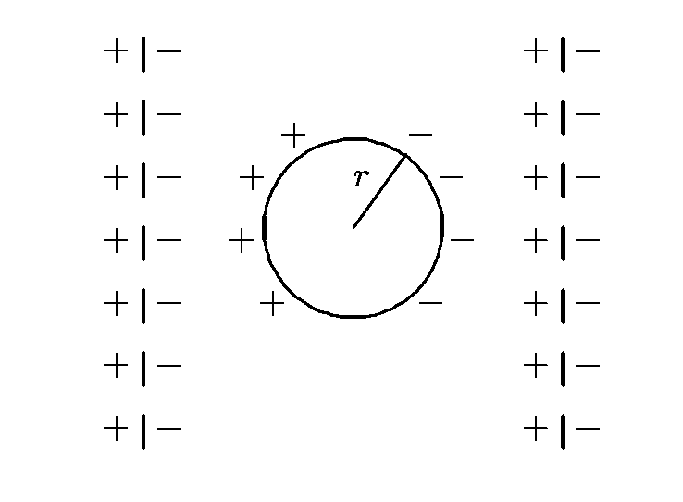
\includegraphics[scale=0.7]{Ris/ris_eps/ris2_01.eps}}}

\risp{1}{К расчету внутреннего
поля} 
\end{figure}

Напряженность действующего на молекулу поля
может быть представлена суммой трех членов:
$$\vec F=\vec F_1+\vec F_2+\vec F_3.\noq$$
Здесь $\vec F_1$ --- поле, создаваемое обкладками конденсатора:
$$\vec F_1=\vec E+4\pi\vec P,$$
где $\vec P$ --- вектор поляризации вещества. $\vec F_2$ --- поле,
обусловленное поляризацией вещества внутри конденсатора, за
вычетом вещества, находящегося внутри сферы. $\vec F_3$ --- поле,
создаваемое молекулами внутри сферы. Существенно, что сфера
мысленно проводится так, чтобы не пересекать ни одной молекулы:
каждая молекула, как целое, участвует в создании либо поля $\vec
F_2$, либо поля $\vec F_3$. Поле $\vec F_2$ в свою очередь состоит
из двух частей: из напряженности, создаваемой слоем зарядов,
индуцированных в диэлектрике у обкладок конденсатора:
$$\vec F'_{2}=-4\pi\vec P,$$
и напряженности поля $\vec F''_{2}$, создаваемого зарядами,
индуцированными на поверхности сферы:
$$\vec F_2=-4\pi\vec P+\vec F''_{2}.$$
Вычислим $\vec F''_{2}$. Плотность заряда на поверхности сферы
равна $P\cos\vartheta$, где $\vartheta$ --- угол между
положительным направлением поля и нормалью в данной точке сферы.
Каждый элемент поверхности сферы $d\Omega$ создает в направлении
поля напряженность, равную в центре сферы радиуса $r$
$${P_n\cos\vartheta\over r^2}d\Omega={P\cos^2\vartheta\over
r^2}d\Omega.$$ Интегрируя по поверхности всей сферы, находим:
$$F''_{2}=\int{P_n\cos\vartheta\over
r^2}d\Omega=\int\limits_0^{\pi}{P\cos^2\vartheta\over r^2}2\pi
r^2\sin\vartheta d\vartheta={4\pi\over3}P,$$ и, следовательно,
$$\vec F_2=-4\pi\vec P+{4\pi\over3}\vec P.$$
Остается вычислить поле $\vec F_3$, создаваемое молекулами,
находящимися внутри сферы. Считаем, что поле каждой молекулы есть
поле диполя. Потенциал в точке $x_0,y_0,z_0$, создаваемый диполем,
находящимся в точке $x,y,z$, отстоящей от $x_0,y_0,z_0$ на $r'$,
равен:
$$\varphi(x_0,y_0,z_0)={\vec p\vec {r'}\over
r'^3}={p_x(x_0-x)+p_y(y_0-y)+p_z(z_0-z)\over r'^3}.$$
Следовательно, в начале координат, в точке $x_0,y_0,z_0=0$ поле
имеет $x$-овую составляющую, равную
$$-\left(\partial\varphi\over\partial
x_0\right)_{x_0,y_0,z_0=0}=-{p_x\over r'^3}+{3\over r'^5}(p_xx^2+
p_yxy+p_zxz).$$ Считая, что диполи во всех молекулах одинаковы,
имеем:
$$\left(F_3\right)_x=p_x\left\{-\left.\sum_k\right.'{1\over
r'^3_k}+\left.\sum_k\right.'{3x_k^2\over
r'^5_k}\right\}+3p_y\left.\sum_k\right.'{x_ky_k\over
r'^5_k}+3p_z\left.\sum_k\right.'{x_kz_k\over r'^5_k}.$$
Суммирование распространяется на все молекулы, находящиеся внутри
сферы, за исключением находящейся в ее центре. При совершенно
хаотическом расположении диполей можем провести усреднение:
$$\left(F_3\right)_x=(N-1)\left[p_x\left\{-\left({\overline{1}\over
r'^3}\right)+\left({\overline{3x^2}\over r'^5}\right)\right\}+p_y
\left({\overline{3xy}\over r'^5}\right)+p_z\left(
{\overline{3xz}\over r'^5}\right)\right].$$ Здесь $N$ --- число
молекул внутри сферы. Так как в изотропном теле
$\overline{x^2}=\overline{y^2}=\overline{z^2}={1\over3}\overline{r'^2}$;
$\overline{xy}=\overline{xz}=\overline{yz}=0$. Получаем $F_3=0$.

Аналогичный результат получается и для кристаллов, принадлежащих с
кубической системе --- оптически изотропных. Итак,
$$\vec F=\vec E+4\pi\vec P-4\pi\vec P+{4\pi\over3}\vec P=\vec
E+{4\pi\over3}\vec P.\noq$$ Мы пришли к этому результату,
рассматривая поведение вещества в электростатическом поле. Однако,
очевидно, что этот вывод в равной степени применим и к переменным
полям, в частности и к полю световой волны. Сопоставляя
соотношения \eqn{13} и
$$\vec D=\varepsilon\vec E=\vec E+4\pi\vec P,\noq$$
находим:
$$\vec F=\vec E+{4\pi\over3}{\varepsilon-1\over4\pi}\vec
E={\varepsilon+2\over3}\vec E={n^2+2\over3}\vec E.\noq$$ Это ---
выражение лорентцова внутреннего поля. Так как, с другой стороны,
$$\vec P=N_1\alpha\vec F,\noq$$
находим из \eqn{13-16}:
$${\varepsilon-1\over\varepsilon+2}={4\pi\over3}N_1\alpha,\noq$$
или
$${n^2-1\over n^2+2}={4\pi\over 3}N_1\alpha. \noq$$
Это соотношение называется формулой Лорентц-Лоренца.

\subzag{Молекулярная рефракция}  Формула Лорентц-Лоренца
\eqn{18} выражает зависимость показателя преломления $n$ от
плотности вещества --- от числа молекул в 1 ${\rm \hbox{см}^3}$ ($N_1$).
Разделив обе части уравнения \eqn{18} на плотность $\rho$ и
умножив их на молекулярный вес вещества, получим в правой части
уравнения величину, не зависящую от плотности, а значит, и от
температуры и давления. Имеем:
$${n^2-1\over
n^2+2}{M\over\rho}={M\over\rho}N_1{4\pi\over3}\alpha=N_A{4\pi\over3}\alpha=R,\noq$$
где $N_A=6,02\cdot10^{23}$ --- число Авогадро, равное числу
молекул в грамм-молекуле. Величина $R$ носит название {\it
молекулярной рефракции}. Ее размерность есть, очевидно,
размерность объема, и так как, в силу сказанного выше, $\alpha$
имеет порядок величины куба линейных размеров молекулы, $R$ должно
по порядку величины совпадать с объемом всех молекул в
грамм-молекуле, рассматриваемых в кинетической теории, как сферы.
Тем самым, порядок величины $R$ есть порядок кубических
сантиметров. Эти рассуждения приводят к выводу, что $R$ должно
совпадать с поправкой на объем в уравнении Ван-дер-Ваальса,
деленной на 4. Приводим некоторые данные (табл. 2.1). 
\begin{figure}[tbp]
\tabp{1}{}

\hbox{\vbox{\halign{\offinterlineskip \vrule\hskip
2mm\strut\hfil #\strut\hfil\hskip2mm &\vrule\hskip 2mm\strut\hfil
#\strut\hfil\hskip2mm &\vrule\hskip 2mm\strut\hfil
#\strut\hfil\hskip2mm &\vrule\hskip 2mm\strut\hfil
#\strut\hfil\hskip2mm &\vrule\hskip 2mm\strut\hfil
#\strut\hfil\hskip2mm & \vrule\hskip 2mm\strut\hfil
#\strut\hfil\hskip2mm & \vrule\hskip 2mm\strut\hfil
#\strut\hfil\hskip2mm &\vrule\hskip 2mm\strut\hfil
#\strut\hfil\hskip2mm \vrule\cr \noalign{\hrule} Вещество&${\rm
H_2}$&${\rm CS_2}$ &${\rm C_6H_{14}}$&${\rm C_6H_6}$&${\rm
H_2O}$&${\rm NH_3}$&${\rm C_6H_5Cl}$\cr\noalign{\hrule} $R,\ {\rm
\hbox{см}^{3}}$&2,0&21,7&29,7&25,9&3,7&5,6&31,1\cr\noalign{\hrule} \vbox
to 4mm {\vskip
0.5mm\hbox{${b\over4}$}}&5,0&19,5&44,0&37,0&7,7&9,5&36,1\cr\noalign{\hrule}
}}} 
\end{figure}

Ввиду простоты и грубости исходных предположений, лучшего
совпадения ожидать не приходится. Независимость молекулярной
рефракции от давления иллюстрируется в табл. 2.2. 
\begin{figure}[tbp]
\tabp{2}{}

\hbox{\vbox{\halign{\vrule\hskip 2mm\strut\hfil
#\strut\hfil\hskip2mm &\vrule\hskip 2mm\strut\hfil
#\strut\hfil\hskip2mm &\vrule\hskip 2mm\strut\hfil
#\strut\hfil\hskip2mm \vrule\cr \noalign{\hrule} Давление,
атм.&$n$&$R,\ {\rm \hbox{см}^{3}}$\cr\noalign{\hrule}
1,00&1,0002929&2,170\cr 28,58&1,008385&2,170\cr
69,24&1,02044&2,180\cr 123,04&1,03633&2,175\cr
176,27&1,05213&2,170\cr\noalign{\hrule} }}} 
\end{figure}

При очень высоких давлениях могут, однако, иметь место
значительные изменения $R$. Это объясняется изменением состояния
электронной оболочки молекулы и, следовательно, величины $\alpha$
в соответствующих условиях.

Практическая независимость молекулярной рефракции от температуры
подтверждается многочисленными опытами. Замечательным фактом
является относительная малость изменений $R$ при изменении
агрегатного состояния вещества, также следующая из формулы
\eqn{19}. Приводим некоторые данные (табл. 2.3).

А. И. Ансельм в своей теории показал, что эллипсоид поляризуемости
молекулы не изменяется при переходе из газа в конденсированную
фазу. Неизменна и оптическая анизотропия молекулы. Но вследствие
того, что в жидкостях существует корреляция в ориентациях
анизотропных молекул, меняются величины, зависящие от анизотропии
поляризуемости: степень деполяризации рассеянного света, константа
Керра и др. 
\begin{figure}[tbp]
\tabp{3}{}

\hbox{\vbox{\halign{\vrule\hskip 2mm\strut\hfil
#\strut\hfil\hskip2mm &\vrule\hskip 2mm\strut\hfil
#\strut\hfil\hskip2mm &\hskip 2mm\strut\hfil #\strut\hfil\hskip2mm
&\vrule\hskip 2mm\strut\hfil #\strut\hfil\hskip2mm &\hskip
2mm\strut\hfil #\strut\hfil\hskip2mm \vrule\cr \noalign{\hrule}
Вещество&\omit\span\omit\vrule \hbox{\hskip 2mm Свойства
жидкости\hskip 2mm}&\omit\span\omit\vrule\hfill\hbox{\hskip 2mm
Свойства газа\hskip 2mm}\hfill\vrule\cr &$n$&$R,\ {\rm
\hbox{см}^{3}}$&$n$&$R,\ {\rm \hbox{см}^{3}}$\cr\noalign{\hrule} $\rm
Br_2$&1,659&9,45&1,000113&8,38\cr $\rm
O_2$&1,221&2,00&1,000271&2,01\cr $\rm
H_2$&1,10&0,92&1,000139&1,02\cr $\rm
N_2$&1,205&2,27&1,000296&2,193\cr $\rm
HCl$&1,245&6,88&1,000447&6,62\cr $\rm
H_2O$&1,334&3,71&1,000249&3,70\cr $\rm
NH_3$&1,325&5,55&1,000373&5,53\cr $\rm
SO_2$&1,410&11,67&1,000690&10,22\cr $\rm
CS_2$&1,628&21,34&1,00147&21,78\cr $\rm
CO_2$&1,192&6,80&1,000449&6,66\cr $\rm
CH_3OH$&1,3308&8,25&1,000549&8,14\cr $\rm
CHCl_3$&1,4467&21,42&1,001436&21,28\cr $\rm
C_2H_5OH$&1,3623&12,76&1,000871&12,92\cr\noalign{\hrule} }}} 
\end{figure}

Все приведенные выше данные относятся к преломлению света с
длинной волны $\lambda=5890\angst$ ($D$-линия Na). Для других
волн, вследствие дисперсии, получатся иные значения $R$, но
практически независимые от плотности и агрегатного состояния
вещества.

Если вещество представляет собой смесь различных молекул, то
молекулярная рефракция смеси аддитивно складывается из рефракций
составляющих веществ.

Пусть в 1 $\rm \hbox{см}^{3}$ смеси содержится $N_1$ молекул первого
сорта, $N_2$ молекул второго сорта и т.д., общее число молекул в 1
$\rm \hbox{см}^{3}$ есть $N$:
$$N=N_1+N_2+...=N(f_1+f_2+...),\noq$$
причем величины
$$f_1={N_1\over N},\ f_2={N_2\over N},\cdots\ ,$$
характеризуют молярные концентрации компонент смеси. Плотность
смеси равна:
$$\rho={N\over N_A}\left(M_1f_1+M_2f_2+...\right)={\overline{M}\over
N_A}N,\noq$$ где $M_1,M_2,...$ --- молекулярные веса компонент
смеси, $\overline{M}$ --- средний молекулярный вес,
$M=M_1f_1+M_2f_2+...$\ . Из простых физических соображений
очевидно, что показатель преломления смеси должен выражаться
уравнением:
$${n^2-1\over
n^2+2}={4\pi\over3}(N_1\alpha_1+N_2\alpha_2+...),\noq$$ где
$\alpha_1,\alpha_2,...$ --- средние поляризуемости различных
веществ, входящих в состав смеси. Умножив \eqn{22} на
${\overline{M}\over \rho}={N_A\over N}$, получим среднюю рефракцию
смеси:
$$\overline{R}={n^2-1\over
n^2+2}{\overline{M}\over\rho}={4\pi\over 3}N_A(f_1\alpha_{1}+
f_2\alpha_2+...)=f_1R_1+f_2R_2+...\ ,\noq$$ что и требовалось
доказать.

Очевидно, что измерение показателя преломления дает возможность
анализа бинарных смесей на основе аддитивности рефракций.
Практически точность определения рефракции лимитируется
погрешностями измерения плотности, значительно более высокими, чем
погрешности при определении $n$. Так, например, при анализе смесей
вода-бензол, погрешность определения концентрации равна $0,008\%$,
для смеси вода-спирт --- $0,04\%$, вода-анилин --- $0,004\%$.
Особенно просты соотношения в случае газов, у которых $n$ близко к
единице. Имеем:
$$R\cong{2\over3}(n-1){M\over\rho}={2\over3}(n-1){N_AkT\over
p},\noq$$ где $k$ --- постоянная Больцмана, $p$ --- давление газа.
Для смеси газов получаем:
$$(n-1)p=(n_1-1)p_1+(n_2-1)p_2+...\ ,\noq$$
где $p_1,p_2,...$ --- парциальные давления. Одновременно
$$p=p_1+p_2+...\ .\noq$$
В случае смеси двух газов из этих уравнений следуют выражения для
объемных концентраций газов:
$${p_1\over p}={n_2-n\over n_2-n_1};\hskip 4mm{p_2\over
p}={n-n_1\over n_2-n_1}.\noq$$ Точность определения количества
$\rm CO_2$ в азоте, проведенного таким методом составляет 0,14\%.


Приведенные в табл. 2.3 оценки точности измерения плотности даны И. В. Обреимовым в 1945 году. В настоящее
время существуют приборы для измерения плотности типа DMA 58. Они позволяют проводить измерения 
с точностью $\pm\cdot 10^{-5} {г\over cм^2}$ в температурной
области от -10° до 70° С и с минимальным объемом образца $\approx 0,7$ мл. Точность внутреннего термостата $\pm 0,005$°C.
Данные приборы запатентованы в Англии, Австрии, Германии и Франции.

\subzag{Аддитивность рефракций гомеополярных соединений} 
Рефракция определенного вещества, и, следовательно, средняя
поляризуемость его молекул, может быть, в ряде случаев,
представлена в виде суммы рефракций, а значит и поляризуемостей
составных частей молекулы. В качестве таких составных частей можно
рассматривать образующие молекулу атомы, ионы или отдельные
валентные связи. Аддитивность имеет место не всегда, но во многих
случаях отклонения от нее незначительны. Этим объясняется большое
значение рефракции при определении структуры молекулы. Химические
свойства молекул определяются свойствами тех валентных связей,
которыми они образованы, и их относительным расположением. Исходя
из идеи аддитивности, получаем возможность зафиксировать те
существенные отклонения от аддитивности --- в частности от
аддитивности рефракций, которые представляют большой интерес,
характеризуя важные группы химических соединений.

Средняя поляризуемость молекулы выражает способность ее
электронной оболочки смещаться под действием внешнего
электрического поля. Электронная оболочка молекулы не может
считаться принадлежащей отдельным атомам. При образовании атомами
различных химических связей, за которые ответственны внешние
электроны, определяющие оптические свойства атомов и молекул,
поляризуемость их электронных оболочек существенно изменяет свой
характер. Так, не следует ожидать одинаковых рефракций у атомов
углерода, образующих единичные, двойные или тройные связи.

Для того, чтобы убедиться в аддитивности молекулярной рефракции,
сопоставим значения этой величины в гомологическом ряду
соединений, в котором каждый последующий член отличается от
предыдущего на одну и ту же группу атомов. Если аддитивность
рефракций действительно имеет место, то разности рефракций любых
двух следующих друг за другом членов ряда должны быть одинаковыми.
Приводим данные для предельных углеводородов нормального строения
(табл. 2.4). 
\begin{figure}[tbp]
\tabp{4}{}

\hbox{\vbox{\halign{\vrule\hskip 2mm\strut\hfil
#\strut\hfil\hskip2mm &\vrule\hskip 2mm\strut\hfil
#\strut\hfil\hskip2mm &\vrule\hskip 2mm\strut\hfil
#\strut\hfil\hskip2mm &\vrule\hskip 2mm\strut\hfil
#\strut\hfil\hskip2mm \vrule\cr \noalign{\hrule}
Вещество&Формула&$R,\ {\rm \hbox{см}^{3}}$&$\Delta R, {\rm
\hbox{см}^{3}}$\cr\noalign{\hrule} н-пентан&$\rm
H_3C-CH_2-CH_2-CH_2-CH_3$&25,28&$-$\cr н-гексан&$\rm
H_3C-(CH_2)_4-CH_3$&29,86&4,58\cr н-гептан&$\rm
H_3C-(CH_2)_5-CH_3$&34,51&4,65\cr н-октан&$\rm
H_3C-(CH_2)_6-CH_3$&39,13&4,62\cr н-нонан&$\rm
H_3C-(CH_2)_7-CH_3$&43,78&4,65\cr н-декан&$\rm
H_3C-(CH_2)_8-CH_3$&48,41&4,63\cr н-ундекан&$\rm
H_3C-(CH_2)_9-CH_3$&53,06&4,65\cr н-додекан&$\rm
H_3C-(CH_2)_{10}-CH_3$&57,67&4,61\cr\noalign{\hrule} }}} 
\end{figure}

Аддитивность действительно имеет место. У изомерных ---
разветвленных предельных углеводородов рефракции не отличаются от
рефракций соответствующих соединений нормального строения. Можно
представить рефракцию предельного углеводорода $\rm C_nH_{2n+2}$ в
виде:
$$R_{C_nH_{2n+2}}=nR_C+(2n+2)R_H.$$
Значит, средняя разность $\Delta R=4,618$, приходящаяся на одну
группу $\rm CH_2$, может быть представлена как
$$4,618=R_C+2R_H.$$
Сопоставляя значение рефракции предельных углеводородов, находим
<< рефракцию углерода>>\ и << рефракцию водорода>>:
$$R_C=2,418{\rm \hbox{см}^{3}}\hskip 4mm;R_H=1,100{\rm \hbox{см}^{3}}.$$
Однако для того же атома углерода, но входящего в состав
непредельного соединения и образующего двойную связь, приходится
вводить другую величину:
$$R_{C=}=4,151 {\rm \hbox{см}^{3}}.$$
Принято говорить, что $R_{C=}$ (или $R_{C\equiv}$ в соединениях
ацетиленового ряда) отличается от $R_{C}$ на величину так
называемого инкремента, инкременты для двойной и тройной связи
обозначаются соответственно значками \inkdu и \inktri. Они имеют
значения:
$$\inkdu=1,733 {\rm \hbox{см}^{3}}\hskip 4mm\inktri=2,398 {\rm \hbox{см}^{3}}.$$
Таким образом,
$$R_{C=}=R_c+\inkdu=2,418+1,733=4,151;$$
$$R_{c\equiv}=R_C+\inktri=2,418+2,398=4,816.$$
Таким образом, рефракция молекулы представляется формулой:
$$R=\sum_nR_n+\sum_iI_i,\noq$$
где первая сумма есть сумма рефракций атомов, а вторая --- сумма
необходимых инкрементов. Введение этих последних свидетельствует о
формальности схемы атомных рефракций. 

Разложение рефракции по
валентным связям физически более обосновано, так как
поляризующиеся электроны локализованы именно на отдельных
валентных связях, образуя их, но не могут быть приписаны отдельным
атомам. При таком разложении необходимость вводить инкременты
отпадает, и выражение молекулярной рефракции представляется в
виде:
$$R=\sum_kR_k,\noq$$
где $R_k$ --- рефракция отдельной связи, и суммирование
распространяется по всем связям в молекуле. Но разложение \eqn{28}
применяется чаще. Формально это приемлемо, так как при наличии
аддитивности \eqn{29} можно с помощью инкрементов установить
однозначное соответствие между атомарными рефракциями и
рефракциями связей. Очевидно, например, что поскольку углерод в
насыщенных соединениях образует четыре валентных связи $\rm C-H$
или четыре валентных связи $\rm C-C$, должно иметь место
соотношение:
\begin{plain}$$\eqalign{R_{C-H}=&{1\over4}R_C+R_H,\cr
R_{C-C}=&{1\over4}R_C+{1\over4}R_C={1\over2}R_C }.$$ \end{plain} Для кратных
связей имеем:
$$R_{C=C}={1\over2}R_C+{1\over2}R_C+\inkdu=R_C+\inkdu,$$
$$R_{C\equiv C}={3\over2}R_C+\inktri,$$
и наоборот:
\begin{plain}$$\eqalign{
R_C=&2R_{C-C},\cr R_H=&R_{C-H}-{1\over2}R_{C-C},}$$
$$\inkdu=R_{C=C}-2R_{C-C},$$
$$\inktri=R_{C\equiv C}-3R_{C-C}.$$
\end{plain}
Значения рефракций атомов и групп с указанием этих величин для
разных длин волн приведены в таблице 7, страница 60 книги <<
Молекулярная оптика>>\ М. В. Волькенштейна. Данные в ней получены
путем сопоставления молекулярных рефракций ряда соединений на
основе аддитивности. Пользуясь данными этой таблицы и ранее
написанными соотношениями, находим:
\begin{plain}$$\eqalign{
R_{C-H}=&1,705;\cr R_{C-C}=&1,209;\cr R_{C=C}=&4,151;\cr
R_{C\equiv C}=&6,025. }$$\end{plain} Все величины для $D$-линии Na. Приведем
таблицу рефракций связей (табл. 2.5). 
\begin{figure}[tbp]
\tabp{5}{}

\hbox{\vbox{\halign{\vrule\hskip 2mm\strut\hfil
#\strut\hfil\hskip2mm &\vrule\hskip 2mm\strut
#\strut\hfil\hskip2mm &\vrule\hskip 2mm\strut\hfil
#\strut\hfil\hskip2mm \vrule\cr \noalign{\hrule} Связь&&$R,\ {\rm
\hbox{см}^{3}}$, D-линия Na\cr\noalign{\hrule} $\rm C-H$&&1,676\cr $\rm
C-C$&&1,296\cr $\rm C=C$&&4,17\cr $\rm C\equiv C$&на конце
цепи&5,87\cr $\rm C\equiv C$&в середине цепи&6,24\cr $\rm C-C$&в
циклопропане&1,49\cr $\rm C-C$&в циклобутане&1,37\cr $\rm C-C$&в
циклопентане&1,26\cr $\rm C-C$&в циклогексане&1,27\cr $\rm C-C$&в
ароматических соединениях&2,688\cr $\rm C-F$&&1,44\cr $\rm
C-Cl$&&6,51\cr $\rm C-J$&&14,61\cr $\rm C-O$&в эфирах&1,54\cr $\rm
C=O$&в метилкетонах&3,49\cr $\rm C-N$&&1,57\cr $\rm C=N$&&3,76\cr
$\rm C\equiv N$&&4,82\cr\noalign{\hrule} }}} 
\end{figure}

\subzag{Рефракция неаддитивных соединений} 

 Для
некоторых групп органических соединений характерно отклонение от
аддитивности рефракций (экзальтация рефракции). В первую очередь
это относится к веществам, содержащим сопряженные двойные связи и
ароматическим соединениям.

Простейшим веществом с сопряженными двойными связями является
бутадиен (дивинил): $\rm H_2C=CH-CH=CH_2$. Его рефракция превышает
вычисленную по аддитивной схеме на $1,42 \rm \hbox{см}^{3}$. Эта величина
носит название экзальтации рефракции:
$$\Delta R=R-\sum_kR_k.\noq$$
Как показывает опыт, экзальтация рефракции тем выше, чем больше
сопряженных связей или ароматических в молекуле ядер содержится.
Понижение симметрии молекулы --- введение метильной группы в
боковую цепочку --- понижает экзальтацию. Например:
\begin{plain}$$\eqalign{
&\hbox{для}\ {\rm H_2C=CH-CH=CH_2}\hskip 4mm \hbox{\ \ }\ \Delta
R=1,42;\cr &\hbox{для}\ {\rm H_2C=\vbox{\hbox{$\rm CH_3$}\vskip
-9.7mm\hbox{$\hskip 1mm |$}\vskip -9mm\hbox{$\rm C$}}\hskip -4mm
-CH=CH_2}\hskip 6.5mm \hbox{\ \ }\ \Delta R=0,88. }$$\end{plain} 

\vskip 8mm
До сих пор не
имеет объяснения факт отсутствия экзальтации у бензола и некоторых
сходных соединений при одновременном большом значении экзальтации
нафталина и последующих членов ряда ароматических соединений:

\vskip 2mm
\centerline{\hbox{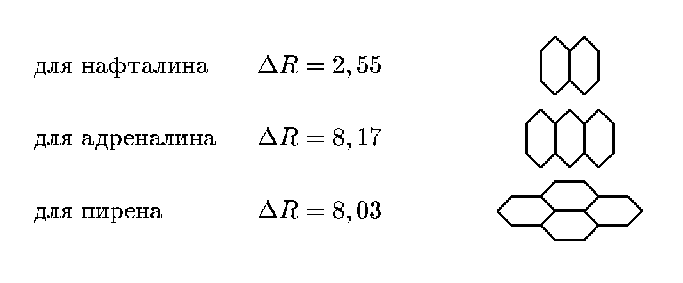
\includegraphics[scale=0.7]{Ris/ris_eps/ris2_01a.eps}}}

\leftskip 0cm Экзальтация может достигать весьма высоких значений,
составляющих существенную долю общей рефракции вещества. Например,
для молекулы мезо-тетрафенилпорфирина $ R=293 \rm \hbox{см}^{3}$, $\Delta
R=90 \rm \hbox{см}^{3}$.

Объяснение этим фактам нужно искать в строении рассматриваемых
молекул. Такие факторы, как сопряжение двойных связей, приводят к
делокализации, обобществлению электронов между связями. В этих
случаях теряет смысл выделение отдельной связи как аддитивной
структурной единицы --- электронная оболочка принадлежит группе
связей или даже всей молекуле. С особенной яркостью эти
обстоятельства проявляются в электронных спектрах поглощения и в
спектрах комбинационного рассеяния.

\subzag{Рефракция ионных соединений}  Для ряда молекул,
которые могут считаться в первом приближении построенными из
ионов, также имеет место аддитивность. Ионные соединения
представляем себе в виде раздельных положительного и
отрицательного ионов, удерживаемых друг около друга на
определенном расстоянии кулоновскими электростатическими силами
притяжения и силами отталкивания. Поэтому следует считать разумным
разложение рефракции ионной молекулы на рефракции ионов.

Однако аддитивность в ионных соединениях соблюдается не строго.
Поляризующиеся электронные оболочки соседних ионов
взаимодействуют. В частности, протон, благодаря своему малому
размеру --- отсутствию внешних электронов --- глубоко проникает в
электронную оболочку аниона и сильно изменяет поляризуемость
последнего, уменьшая ее.

Сопоставим рефракции следующих изоэлектронных соединений: \vskip
1mm \hfil\hbox{\vbox{\halign{\vrule\hskip 2mm\strut\hfil
#\strut\hfil\hskip2mm &\hskip 2mm\strut\hfil #\strut\hfil\hskip2mm
&\vrule\hskip 2mm\strut\hfil #\strut\hfil\hskip2mm &\hskip
2mm\strut\hfil #\strut\hfil\hskip2mm \vrule\cr \noalign{\hrule}
$\rm Cl^-$&9,30&HCl&6,67\cr $Br^-$&12,04&HBr&9,19\cr
$J^-$&19,07&HJ&13,74\cr\noalign{\hrule} }}}\hfill

Упрощенные электростатические представления вынуждают вводить при
расчете рефракции неорганических соединений различные поправки на
взаимодействие ионов между собой и на влияние окружающей среды.
Например, рефракция иона $\rm Cl^-$, определяемая из соединений
$\rm NaCl$, $\rm MgCl_2$, $\rm AlCl_3$, $\rm SiCl_4$, $\rm PCl_5$,
различна не вследствие различий во взаимной поляризации, которые
могут быть учтены простым электростатическим расчетом. В
действительности, в указанном ряду меняется характер химической
связи, становящейся при переходе слева направо все более
гомеополярной.

Из всего вышеизложенного следует, что схема аддитивности ионных
рефракций применима только как первое приближение, полезное для
целей предварительной ориентировки.

\subzag{Определение показателя преломления методом предельного
угла}  Если луч света пересекает границу раздела двух
прозрачных однородных сред 1 и 2 (рис. 2.2), то направление луча
изменяется в соответствии с установленным еще в начале XVII века
законом преломления. Согласно этому закону, отношение синусов
углов падения $i_1$ и преломления $i_2$ есть величина постоянная:
$${\sin i_1\over\sin i_2}=n_{12}.\noq$$

\begin{figure}[tbp]
\centerline{\hbox{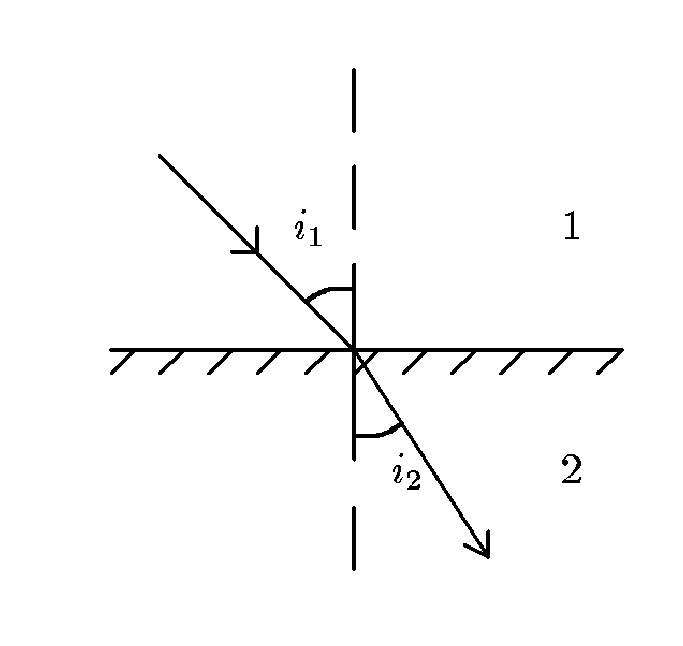
\includegraphics[scale=0.7]{Ris/ris_eps/ris2_02.eps}}}

\risp{2}{Преломление луча на
границе двух прозрачных сред} 
\end{figure}

 Константа $n_{12}$
называется относительным показателем (или коэффициентом)
преломления второго вещества по отношению к первому.

Волновая теория света устанавливает простую связь показателя
преломления со скоростью распространения световых волн в двух
средах $v_1$ и $v_2$:
$$n_{12}={v_1\over v_2}.\noq$$
Показатель преломления по отношению к << пустоте>>\ называется
абсолютным показателем преломления. Из формулы \eqn{32} следует,
что абсолютный показатель преломления вещества $n$ равен отношению
скорости света в пустоте $c=3\cdot10^{10}$ см/сек к скорости света
в веществе $v$:
$$n={c\over v}.\noq$$
Относительный показатель преломления $n_{12}$ согласно \eqn{32} и
\eqn{33}, равен отношению абсолютных показателей преломления
веществ 1 и 2:
$$n_{12}={n_2\over n_1}.\noq$$
Принимая во внимание это соотношение, закон преломления \eqn{31}
можно записать в удобной для запоминания форме:
$$n_1\sin i_1=n_2\sin i_2.$$

При измерении показателей преломления жидких и твердых тел обычно
определяются их относительные показатели преломления по отношению
к воздуху лабораторного помещения.

Показатели преломления по отношению к воздуху в химической
рефрактометрии просто называют показателями преломления и
обозначают буквой $n$. Абсолютные показатели преломления
обозначают {\bfseries n}. Соотношение между {\bfseries n} и $n$,
согласно определению этих величин и формуле \eqn{34}, следующее:
$$\hbox{\bfseries n}=\hbox{\bfseries n}_{\rm \hbox{воздуха}}\cdot n.\noq$$
Таким образом, для получения абсолютных показателей преломления
достаточно умножить определяемые при обычных рефрактометрических
измерениях величины на абсолютный показатель преломления воздуха.

При нормальном атмосферном давлении и комнатной температуре
$\hbox{\bfseries n}_{\rm \hbox{воздуха}}=1,00027$, следовательно:
$$\hbox{\bfseries n}=1,00027\cdot n.\noq$$
Соотношение \eqn{36} --- приближенное, так как не учитывает
зависимости абсолютного показателя преломления воздуха от
давления, температуры и влажности. В подавляющем большинстве
случаев, когда не требуется абсолютной точности измерения n,
превышающей $1\cdot10^{-4}$, такое упрощение вполне допустимо.

Показатель преломления вещества определяется его природой, но
зависит также от внешних условий (главным образом от температуры и
от длины волны света). Длину волны указывают подстрочным индексом,
а температуру --- надстрочным индексом справа. Например, символ
$n_{480}^{25}$ обозначает показатель преломления при 25$^{\circ}$C
для голубой линии кадмия с длиной волны 480 нм ($4800 \angst$).
Вместо длины волны часто употребляемых спектральных линий обычно
указывают их буквенные обозначения. Так, например, $n_{D}^{20}$,
$n_C^{20}$ и $n_F^{20}$ обозначают показатели преломления при
20$^{\circ}$C для линии $D$ натрия (5893\angst) и линий $C$ и $F$
водорода ($\lambda_C=6563\angst,\ \lambda_F=4861\angst$).

У оптически анизотропных веществ, к которым относится большинство
кристаллов (кроме кристаллов кубической системы), наблюдается
двойное лучепреломление --- расщепление преломляющегося луча на
два луча, распространяющихся с разными скоростями. При этом у так
называемых одноосных кристаллов (гексагональной, тетрагональной и
тригональной систем) скорость распространения одного из лучей,
называемого необыкновенным, зависит от его направления. В
оптически двуосных кристаллах низкой симметрии (ромбической,
моноклинной и триклинной систем) скорость распространения обоих
преломленных лучей зависит от направления. В связи с этим
оптически анизотропные вещества характеризуются двумя
экстремальными показателями $n_{o}$ и $n_{e}$ (одноосные
кристаллы) или тремя показателями $n_p,n_m,n_g$ (двуосные
кристаллы). В данном случае индексы $o$ и $e$ относятся к
обыкновенному и необыкновенному лучам, а индексы $p,\ g$ и $m$
обозначают соответственно наименьший, наибольший и промежуточный
показатели преломления в трех взаимно перпендикулярных
направлениях.

Согласно закону преломления света \eqn{31}, при $n_{12}={n_2\over
n_1}>1$, $\sin i_1>\sin i_2$, и, следовательно, $i_1>i_2$. Отсюда
следует, что при преломлении света угол $i_2$ не может быть больше
некоторой величины $\varphi<90^{\circ}$, соответствующей
$i_1=90^{\circ}$ и определяемой непосредственно вытекающим из
закона преломления соотношением:
$$\sin\varphi={n_1\over n_2}.\noq$$
Как показывает опыт, луч, падающий из среды с большим показателем
преломления на границу раздела с менее преломляющей средой под
углом $i_2>\varphi$, не преломляется, а полностью отражается (рис.
2.3). Это явление, называемое полным внутренним отражением, было
известно давно и отмечено Кеплером еще до открытия закона
преломления света.

\begin{figure}[tbp]
\centerline{\hbox{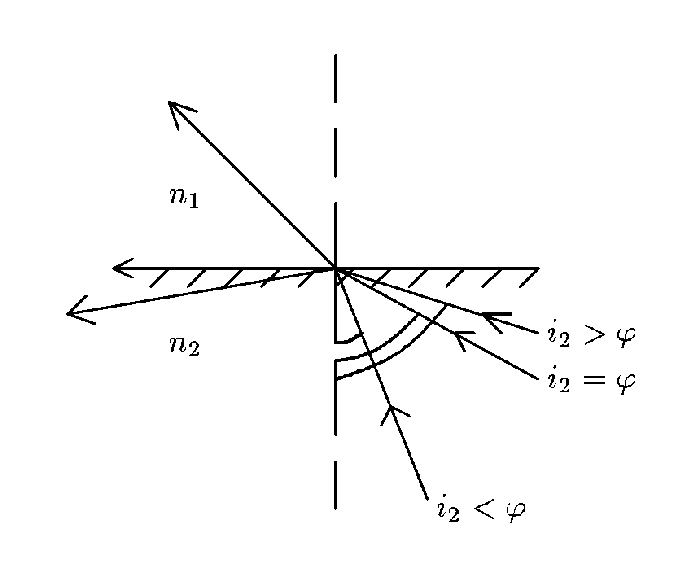
\includegraphics[scale=0.7]{Ris/ris_eps/ris2_03.eps}}}

\risp{3}{Полное внутреннее
отражение} \vskip 0.5mm \noindent{\Small Лучи, падающие на границу
раздела из более преломляющей среды (${\mitsm n_1<n_2}$) под
углом, превышающим ${\mitsm\varphi}$ (предельный угол), полностью
отражаются от границы раздела.} 
\end{figure}

При $i_2<\varphi$
происходит преломление луча, сопровождающееся частичным отражением
от границы раздела. Предельное значение $i_2=\varphi$ называется
предельным, или критическим углом.

Предельный угол можно измерять двумя способами. Во-первых, можно
направить на границу раздела пучок лучей со стороны среды с
большим показателем преломления под углом, близким к предельному,
и наблюдать отраженный свет, как показано на рис. 2.4а. Во-вторых,
можно осветить границу раздела сред скользящим пучком лучей со
стороны слабопреломляющей среды и рассматривать преломленные лучи
(рис. 2.4б). В обоих случаях наблюдается граница светотени,
соответствующая предельному углу. Второй способ (способ <<
скользящего вхождения лучей>>\ или способ << работы в проходящем
свете>>) дает очень отчетливую и контрастную границу, но пригоден
только для прозрачных сред. Первый из этих способов (работа в
отраженном свете) может применяться и в том случае, когда
слабопреломляющая среда малопрозрачна, но дает небольшую разницу
освещенностей светлой и затемненной частей поля зрения, так что
граница наблюдается труднее.

Для наблюдения предельного угла на плоской границе между двумя
твердыми телами необходимо устранить тончайшую прослойку воздуха,
которая остается между полированными поверхностями твердых тел при
простом наложении их друг на друга. Устранения воздушной прослойки
достигают, раздавливая между складываемыми гранями каплю жидкости
с высоким показателем преломления, так называемой контактной
жидкости. Показатель преломления контактной жидкости должен быть
больше, чем у твердого тела, в противном случае наблюдаемый
предельный угол будет соответствовать полному внутреннему
отражению на границе жидкости и твердого тела, а не на границе
двух твердых тел.

\begin{figure}[tbp]
\centerline{\hbox{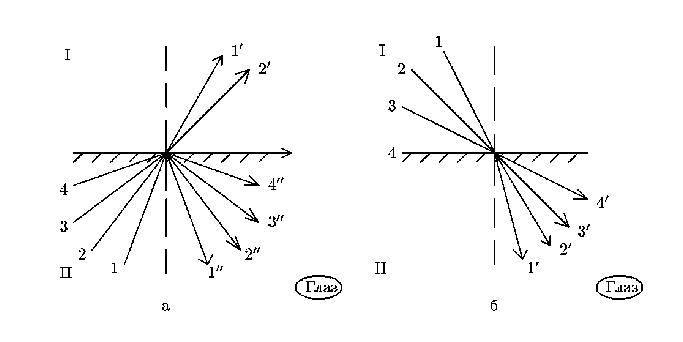
\includegraphics[scale=0.7]{Ris/ris_eps/ris2_04.eps}}}

\risp{4}{ Два способа наблюдения
предельного угла}

\noindent{\Small а --- в отраженном свете, б --- в проходящем
свете. I --- среда с меньшим показателем преломления; II --- среда
с большим показателем преломления.} 
\end{figure}

Непосредственный
оптический контакт между поверхностями двух твердых тел может быть
достигнут, если одна из этих поверхностей плоская, а другая слабо
выпуклая. При сдавливании таких поверхностей возникают кольца
Ньютона, причем на центральном пятне можно наблюдать полное
внутреннее отражение без контактной жидкости. Такой метод
наблюдения полного внутреннего отражения может быть полезен при
измерении показателей преломления сильнопреломляющих твердых тел,
когда трудно подыскать контактную жидкость с достаточно высоким
показателем преломления.

Величина предельного угла на границе двух веществ зависит только
от показателей преломления этих веществ. Следовательно, если
известен показатель преломления одного вещества, то показатель
преломления другого вещества можно определить, измерив предельный
угол $\varphi$:
$$n_1=n_2\sin\varphi.\noq$$
Удобство этого способа состоит в том, что требуется измерение
только одного угла, а исследуемому телу не надо придавать строго
определенную геометрическую форму, так как для наблюдения полного
внутреннего отражения существенно лишь наличие плоской границы
раздела.

Измерение предельного угла для определения показателей преломления
было, по видимому, впервые использовано Волластоном в начале XIX
в. С конца XIX в., когда были созданы удобные конструкции
специальных рефрактометров, метод предельного угла получил широкое
распространение и в настоящее время служит важнейшим способом
измерения показателей преломления в химических приложениях
рефрактометрии.

Существенной деталью большинства рефрактометров, основанных на
определении предельного угла, является измерительная призма из
оптического стекла с точно известным показателем преломления N.
Одна из граней измерительной призмы (так называемая входная грань)
приводится в оптический контакт с измеряемым телом и служит
границей раздела, на которой происходит преломление и полное
внутреннее отражение. Преломление или отражение света на этой
грани наблюдается в зрительную трубу обычно через вторую
(выходную) грань призмы (рис. 2.5).

\begin{figure}[tbp]
\centerline{\hbox{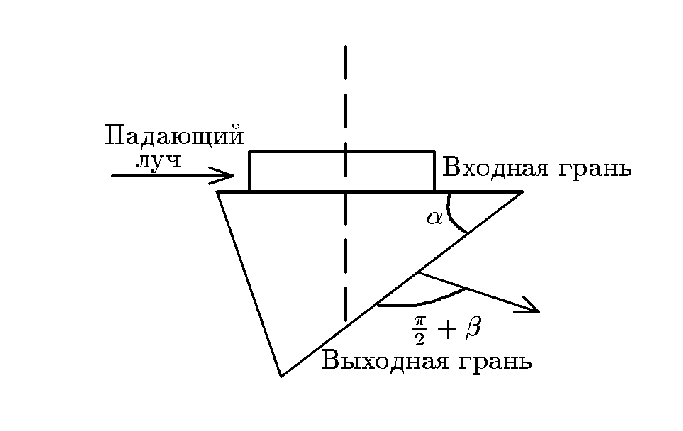
\includegraphics[scale=0.7]{Ris/ris_eps/ris2_05.eps}}}

\risp{5}{Принципиальная схема
рефрактометра, основанного на измерении } 
\centerline{\small предельного угла} 
\end{figure}


Как сказано выше, угол $\alpha$ между входной и выходной
гранями называется преломляющим углом призмы. Луч, соответствующий
предельному углу $\varphi$ и называемый предельным лучом, после
преломления на границе стекло призмы --- воздух составляет с
нормалью к выходной грани некоторый угол $\beta$.

При рассматривании вышедших из призмы лучей, близких к
предельному, поле зрения трубы оказывается разделенным на
освещенную и темную части, граница между которыми соответствует
предельному лучу.

Разные типы рефрактометров предельного угла отличаются величиной
преломляющего угла измерительных призм, величиной их показателей
преломления, конструкцией угломерных устройств и применяемыми
источниками света.

Каждый рефрактометр предельного луча пригоден для измерения
показателей преломления только в определенных пределах их значений
и в этом отношении не является прибором вполне универсальным.
Верхний предел измеряемых показателей преломления $n$ зависит от
показателя преломления стекла измерительной призмы $N$. Нетрудно
видеть, что при показанном на рис. 2.5 способе наблюдения
предельного луча должно соблюдаться неравенство $n<N$, т.е.
измеряемый показатель преломления должен быть меньше показателя
преломления призмы. Нижний предел измеряемых $n$ зависит от
конструкции прибора (угла $\alpha$, размеров призм, угломерного
устройства).

Как следует из изложенного, в методе предельного угла измеряется
обычно не непосредственно предельный угол $\varphi$, а угол
$\beta$ между предельным лучом и нормалью к выходной грани.

Формулу, связывающую величину угла $\beta$ с показателем
преломления исследуемого вещества $n$, нетрудно получить,
рассматривая преломление предельного луча на гранях призмы. Для
полного внутреннего отражения на входной грани имеем соотношение:
$$\sin\varphi={n\over N},\noq$$
а для преломления на выходной грани:
$$\sin\beta=N\sin\beta',\noq$$
причем
$$\beta'=\pm(\varphi-\alpha)\ \ \hbox{или}\ \
\varphi=\alpha\pm\beta'.\noq$$ Знак << плюс>>\ в уравнениях
\eqn{34} относится к случаю, когда предельный луч выходит от
нормали в сторону преломляющего ребра призмы, как на рис. 2.5, а
знак << минус>>\ --- когда предельный луч располагается по
другую сторону нормали. Исключая промежуточные углы $\beta'$ и
$\varphi$ из уравнений \eqn{39-41}, получим:
$$n=\sin\alpha\left(\sqrt{N^2-\sin^2\beta}\right)\pm\cos\alpha\sin\beta.\noq$$
Эта формула лежит в основе всех расчетов при измерениях методом
предельного угла на призме. По формуле \eqn{42} производятся
вычисления показателей преломления $n$, расчеты шкал
рефрактометров и вспомогательных таблиц к ним.

Дифференцируя \eqn{42} по $N$, $\alpha$ или $\beta$, нетрудно
получить соотношения, необходимые для учета возможных погрешностей
измерений. Наиболее важным из них является соотношение для учета
несоответствия истинного значения показателя преломления стекла
призмы принимаемому при расчете значению $N$. Ошибка $\Delta N$
повлечет за собой ошибку в определении $n$, равную:
$$\Delta n={N\sin\alpha\over\sqrt{N^2-\sin^2\beta}}\Delta N.\noq$$
Формула \eqn{43} используется, в частности, для внесения
температурных поправок, когда $\Delta N$ вызывается отклонением
температуры призмы от стандартной.

Неточность преломляющего угла призмы $\Delta \alpha$ вызовет
ошибку измерения показателя преломления $\Delta n$:
$$\Delta
n=\left(\cos\alpha\left(\sqrt{N^2-\sin^2\beta}\right)-\sin\beta\sin\alpha
\right)\Delta\alpha=\left(\sqrt{N^2-n^2}\right)\Delta\alpha.\noq$$
Наконец, угломерная ошибка $\Delta\beta$ приведет к ошибке $\Delta
n$, равной:
$$\Delta
n={\cos^2\beta\sqrt{N^2-n^2}\over\sqrt{N^2-\sin^2\beta}}\Delta\beta.\noq$$

\subzag{Рефрактометры типа Пульфриха. ИРФ-23} 
Рефрактометр Пульфриха --- основной прибор, применяемый для
специальных исследовательских работ в области химических
приложений рефрактометрии.

Характерной особенность рефрактометров Пульфриха является
использование источников света с линейчатым спектром и
измерительных призм с преломляющим углом 90$^{\circ}$. Принцип
действия прибора основан на явлениях, происходящих при прохождении
света через границу раздела двух сред с разными показателями
преломления. Подставив $\alpha=90^{\circ}$ в основную формулу,
получим формулу для определения показателя преломления на
рефрактометрах данного типа:
$$n=\sqrt{N^2-\sin^2\beta}.\noq$$
если скользящий луч, падающий из среды с меньшим показателем
преломления $n$, отклонить до предела и пустить вдоль поверхности
второй среды под углом $90^{\circ}$ с нормалью, то во второй среде
с большим показателем преломления $N$ он выйдет под углом $\beta$.
Ход лучей в призме рефрактометра Пульфриха схематически показан на
рис. 2.6.

\begin{figure}[tbp]
\centerline{\hbox{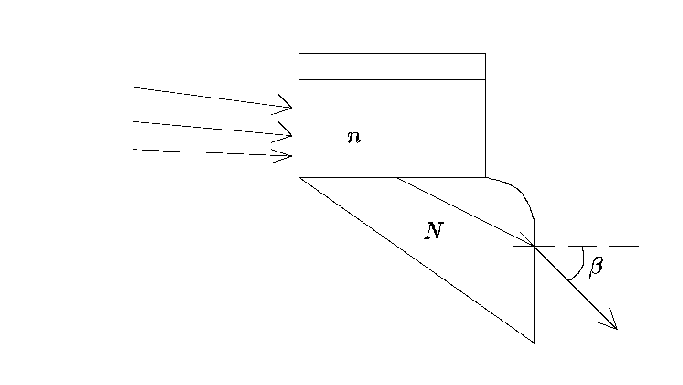
\includegraphics[scale=0.7]{Ris/ris_eps/ris2_06.eps}}}

\risp{6}{Ход лучей в измерительной
призме рефрактометра Пульфриха} 
\end{figure}

Рефрактометр снабжен
набором измерительных призм, из которых всегда можно выбрать
призму с показателем преломления большим, чем у измеряемого
вещества.

На приборе определяются показатели преломления прозрачных жидких и
твердых веществ. В первом случае исследуемая жидкость наливается в
стаканчик, который предварительно приклеивается к измерительной
призме прибора. Конструктивно измерительная призма выполнена так,
что место склейки ее со стаканчиком находится ниже ее верхней
грани и не мешает прохождению лучей. Края верхней грани призмы
сошлифованы по сфере, так что входная грань имеет форму круга,
радиус которого несколько меньше внутреннего радиуса стаканчика.
Нижняя часть стаканчика также имеет сферический шлиф, притертый по
сферической части призмы.

При испытании твердых тел исследуемый образец, имеющий две плоские
полированные поверхности, расположенные под прямым углом,
накладывается на верхнюю грань измерительной призмы. При этом
между соприкасающимися поверхностями образца и призмы помещается
тонкий слой (одна капля) жидкости с показателем преломления,
превышающим показатель преломления исследуемого образца, но не
превышающим показатель преломления измерительной призмы.

Устройство для измерения угла $\beta$ состоит из зрительной трубы,
наглухо соединенной со стеклянным лимбом, закрытым металлическим
кожухом, и спирального микрометра. В окуляре микрометра имеется
вертикальная шкала с десятью делениями, каждое из которых
соответствует 0,1$^{\circ}$. Сотые и тысячные доли градуса
определяются при помощи вращающейся спирали с двойными витками.
Шаг этой спирали (смещение при полном обороте) точно равен
расстоянию между делениями окулярной шкалы, т.е. соответствует
$0,001^{\circ}$. Маховичком вращают спираль до тех пор, пока
градусный штрих лимба не расположится симметрично между двойными
штрихами витка спирали. Номер этого градусного штриха дает число
целых градусов. Десятые доли определяются числом целых делений
окулярной шкалы, пройденных градусным штрихом лимба. Сотые и
тысячные доли отсчитывают против индекса на кольцевой шкале
спирали.

Таким образом, точность и удобство измерений углов значительно
повышаются и отпадает необходимость в отдельной шкале
микрометрического винта для дифференциальных измерений.
Микрометрический винт служит в приборе только для точной наводки
трубы.

В фокальной плоскости окуляра трубы расположен визирный крест,
наводимый при измерениях на границу внутреннего отражения. При
рассматривании границы полного внутреннего отражения в трубу
наблюдается ряд спектральных полос, ширина которых зависит от
положения диафрагмы конденсатора, ограничивающей сверху пучок
падающих на призму лучей. Поворотом диафрагмы можно регулировать
ширину полос и добиться разделения близко расположенных
спектральных линий.

Взаимное расположение спектральных полос зависит от соотношения
численных значений дисперсий измеряемого вещества и стекла призмы.
Чем больше они различаются, тем больше видимое расстояние между
полосами. Обычно дисперсия измеряемого вещества меньше дисперсии
стекла призмы, и вверху поля зрения располагаются красные линии, а
внизу --- синие и фиолетовые. Обратное (необычное) расположение
линий имеет место, когда дисперсия вещества больше дисперсии
призмы. Чтобы измерить угол $\beta$, надо навести крест на верхнюю
(резкую) границу спектральной полосы и произвести отсчет по лимбу
и спиральному микрометру. Распространенной ошибкой является
установка креста не на верхнюю границу, а на середину спектральной
полосы. Ширина спектральной полосы, а следовательно, и положение
ее середины зависит от положения диафрагмы конденсатора.
Результаты измерений при такой неправильной установке креста будут
ниже истинных значений показателей преломления. К рефрактометру
Пульфриха прилагается несколько призм, каждая из которых
предназначается для измерений в определенных пределах $n$. Полный
комплект к прибору ИРФ-23 состоит из трех призм. Призма № 1
изготавливается из флинта Ф-2 ($N_D=1,617$) и предназначена для
работы с жидкими и твердыми образцами, имеющими $n=1,31\div 1,61$.
Призма № 2 сделана из тяжелого флинта ТФ-4 ($N_D=1,740$) и
позволяет измерять $n=1,46\div 1,73$. Призма № 3 делается из
стекла ТФ-10 с очень высоким показателем преломления ($N_D=1,806$
и служит для измерения $n$ некоторых сильно преломляющих стекол и
неорганических жидкостей, не укладывающихся в интервал показателей
призмы № 2 ($n=1,54\div 1,80$).

К каждой призме имеется таблица для перевода углов $\beta$ в
показатели преломления, рассчитанная по формуле \eqn{46}. Точные
значения показателей преломления призм, изготовленных в разное
время из стекла разных варок, несколько различаются и гравируются
на матовой части верхней поверхности призм. Следует обращать
внимание на соответствие указанных в таблицах значений показателей
преломления выгравированным на самих призмах.

\markright{\hfill\small Интерференционно-поляризационный метод измерения\hfill}
\subzag{Интерференционно-поляризационный метод измерения разности
показателей преломления}  

\markright{\hfill\small Интерференционно-поляризационный метод измерения\hfill}

Сущность
интерференционно-поляризационного метода измерения разности
показателей преломления заключается в поляриметрическом
определении разности хода двух лучей со взаимно ортогональными
плоскостями поляризации, интерферирующими после прохождения через
среды с показателями преломления $n_1$ и $n_2$.

Академик Лебедев одним из первых практически применил схему
поляризационного интерферометра для определения под микроскопом
показателя преломления микроскопических зерен и оптических
неоднородностей в оптических стеклах, а также в тонких
биологических срезах. Затем модификация схемы Лебедева была
использована в микрорефрактометре Захарьевского.

На рис. 2.7 показана принципиальная схема
интерференционно-поляризационного рефрактометра.
Плоскополяризованный пучок света разделяется с помощью
поляризационного элемента (кристалл кварца или исландского шпата)
на два когерентных пучка равной интенсивности, поляризованных во
взаимноортогональных плоскостях.

\begin{figure}[tbp]
\centerline{\hbox{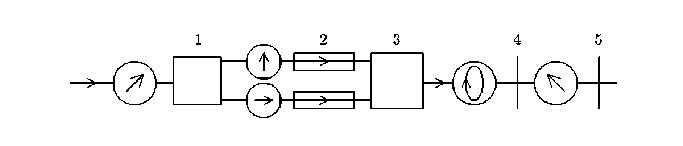
\includegraphics[scale=0.7]{Ris/ris_eps/ris2_07.eps}}}

\risp{7}{Принципиальная схема
интерференционно-поляризационного рефрактометра}

\noindent{\Small 1,3 --- поляризационные элементы, 2 --- кюветы со
сравниваемыми веществами, 4 --- пластинка << в четверть длины
волны>>, 5 --- анализатор.} 
\end{figure}

На пути пучков помещается
кювета 2 со сравниваемыми веществами. Сведение пучков
осуществляется аналогичным поляризационным элементом 3. Суммарная
разность хода $\Delta_{\Sigma}$ после сведения пучков определяется
выражением:
$$\Delta_{\Sigma}=2\Delta+(n_2-n_1)l.\noq$$
Величина вносимой каждым поляризационным элементом разности хода
$\Delta$ является постоянной при достаточной температурной и
механической стабилизации поляризационных элементов и может быть
либо скомпенсирована, либо при достаточной временной когерентности
используемого излучения просто исключена из рассмотрения как
постоянная составляющая. Таким образом, можно считать, что при
данной длине кюветы $\Delta_{\Sigma}$ определяется только
величиной $n_2-n_1=\Delta n$, которой соответствует разность фаз
$\delta$:
$$\delta={2\pi\over\lambda}\Delta n\cdot l.\noq$$
Световые пучки равной интенсивности с разностью фаз $\delta$,
складываясь во втором поляризационном элементе, главное
направление которого ориентировано параллельно главному
направлению первого, дают эллиптически поляризованную волну,
причем большая ось эллипса либо параллельна, либо перпендикулярна
плоскости поляризации падающего света. Фазовая пластинка << в
четверть длины волны>>\ 4 с главными направлениями,
ориентированными параллельно осям эллипса, преобразуют
эллиптическое колебание в плоскополяризованное. Плоскость
поляризации выходящего из фазовой пластинки луча повернута
относительно первоначального плоскополяризованного луча на угол
$\psi={\delta\over2}$, связанный, согласно \eqn{48}, с разностью
показателей преломления $n_1$ и $n_2$ соотношением:
$$\Delta n={\lambda\over\pi l}\psi.\noq$$
Угол $\psi$ с помощью анализатора 5 может измеряться с точностью
до $0,001^{\circ}$, что при малой величине отношения
${\lambda\over l}$ обеспечивает высокую чувствительность
интерференционно-поляризационного метода.

Анализируя формулу \eqn{49} для сопоставления данных
интерференционно-поляризационного метода с аналогичными
параметрами интерферометра Рэлея, находим, что чувствительность
описываемого метода выше на четыре порядка, что позволяет с
миллиметровой кюветой достигнуть чувствительности измерения
вдесятеро более высокой, чем на метровой кювете обычного
лабораторного интерферометра. Высокая чувствительность
интерференционно-поляризационного метода нашла практическое
применение при изучении диффузионных процессов.


\vskip 5 mm
\noindent{\bfseries Литература к главе:}
\vskip 2 mm
1. {\itshape Лорентц.} Теория электронов. ОНТИ. 1935 г. 

2. {\itshape А. И. Ансельм.} ЖЭТФ. $\underline{17}$. 489. 1947 г.

3. {\itshape И. В. Обреимов.} О приложении френелеой диффрации для физических и технических измерений АНСССР. 1945 г.

4. {\itshape Б. В. Иоффе.} Рефрактометрические методы в химии. Л. 1974 г.

5. {\itshape М. Ф. Вукс.} Рассеяние света в газах, жидкостях и растворах. ЛГУ, 1977.

6. {\itshape Е. И. Бутиков, В. А. Замков, А. С. Кондратьев.} Исследование чувствительности и устойчивости
поляризационного интерферометра Дайсона. ОМП. 1975. vol. 42 №7.

7. Описание прибора для точного измерения плотности DMA-58.

